\documentclass[10pt]{book}

%These tell TeX which packages to use.
\usepackage{array,epsfig}
\usepackage{amsmath}
\usepackage{amsfonts}
\usepackage{amssymb}
\usepackage{amsxtra}
\usepackage{amsthm}
\usepackage{mathrsfs}
\usepackage{color}
\usepackage{enumitem}
%\usepackage{mdframed}
\usepackage[most]{tcolorbox}
\usepackage{pgfplots}
\usetikzlibrary{arrows}
\pgfplotsset{compat=1.6}

\pgfplotsset{soldot/.style={color=black,only marks,mark=*}} \pgfplotsset{holdot/.style={color=black,fill=white,only marks,mark=*}}

%Here I define some theorem styles and shortcut commands for symbols I use often
\theoremstyle{definition}
\newtheorem{defn}{Definition}
\newtheorem{thm}{Theorem}
\newtheorem{cor}{Corollary}
\newtheorem*{rmk}{Remark}
\newtheorem{lem}{Lemma}
\newtheorem*{joke}{Joke}
\newtheorem{ex}{Example}
\newtheorem*{soln}{Solution}
\newtheorem{prop}{Proposition}

\newcommand{\lra}{\longrightarrow}
\newcommand{\ra}{\rightarrow}
\newcommand{\surj}{\twoheadrightarrow}
\newcommand{\graph}{\mathrm{graph}}
\newcommand{\bb}[1]{\mathbb{#1}}
\newcommand{\Z}{\bb{Z}}
\newcommand{\Q}{\bb{Q}}
\newcommand{\R}{\bb{R}}
\newcommand{\C}{\bb{C}}
\newcommand{\N}{\bb{N}}
\newcommand{\M}{\mathbf{M}}
\newcommand{\m}{\mathbf{m}}
\newcommand{\MM}{\mathscr{M}}
\newcommand{\HH}{\mathscr{H}}
\newcommand{\Om}{\Omega}
\newcommand{\Ho}{\in\HH(\Om)}
\newcommand{\bd}{\partial}
\newcommand{\del}{\partial}
\newcommand{\bardel}{\overline\partial}
\newcommand{\textdf}[1]{\textbf{\textsf{#1}}\index{#1}}
\newcommand{\img}{\mathrm{img}}
\newcommand{\ip}[2]{\left\langle{#1},{#2}\right\rangle}
\newcommand{\inter}[1]{\mathrm{int}{#1}}
\newcommand{\exter}[1]{\mathrm{ext}{#1}}
\newcommand{\cl}[1]{\mathrm{cl}{#1}}
\newcommand{\ds}{\displaystyle}
\newcommand{\vol}{\mathrm{vol}}
\newcommand{\cnt}{\mathrm{ct}}
\newcommand{\osc}{\mathrm{osc}}
\newcommand{\LL}{\mathbf{L}}
\newcommand{\UU}{\mathbf{U}}
\newcommand{\support}{\mathrm{support}}
\newcommand{\AND}{\;\wedge\;}
\newcommand{\OR}{\;\vee\;}
\newcommand{\Oset}{\varnothing}
\newcommand{\st}{\ni}
\newcommand{\wh}{\widehat}
%Pagination stuff.
\setlength{\topmargin}{-0.75in}
\setlength{\oddsidemargin}{0in}
\setlength{\evensidemargin}{0in}
\setlength{\textheight}{9.in}
\setlength{\textwidth}{6.5in}
\pagestyle{empty}
\begin{document}
\begin{flushleft}
Name:\underline{\hspace{13cm}}Date:\underline{\hspace{2cm}}
\end{flushleft}
\begin{center}
{\Large Math 1041-012 \hspace{0.5cm} Section 4.2}
\end{center}
%\vspace{0.2 cm}

\begin{tcolorbox}
\subsection*{Rolle's Theorem}
Let $f$ be a function such that
\begin{enumerate}
    \item $f$ is \underline{\hspace{3cm}} on the closed interval $[a,b]$,
    \item $f$ is \underline{\hspace{3cm}} on the open interval $(a,b)$,
    \item and \underline{\hspace{3cm}}
\end{enumerate}
then the conclusion is: there is a number $c$ in $(a,b)$ such that $f'(c)=0$.\\ \\
\textit{In other words}: if you have a continuous differentiable function on a closed interval where the endpoints have the same $y$ value, then somewhere in your interval you have of tangent slope of 0.\\ \\
With the above hypothesis, we are guaranteed AT LEAST ONE location in an open interval where the curve has tangent slope of zero.
\end{tcolorbox}
There are many ways that we can visualize this:\\
\begin{figure}[h]
    \centering
    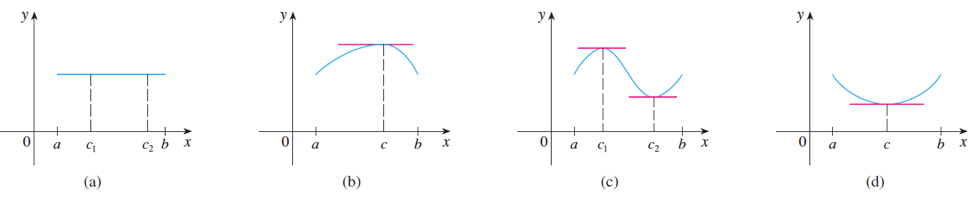
\includegraphics{RollesTheorem.png}
\end{figure}
\subsection*{Example 1} The graph of $f$ is shown below. Verify that $f$ satisfies the hypotheses of Rolle's Theorem. Then estimate the value(s) of $c$ that satisfy the conclusion of Rolle's Theorem.
\begin{figure}[h]
    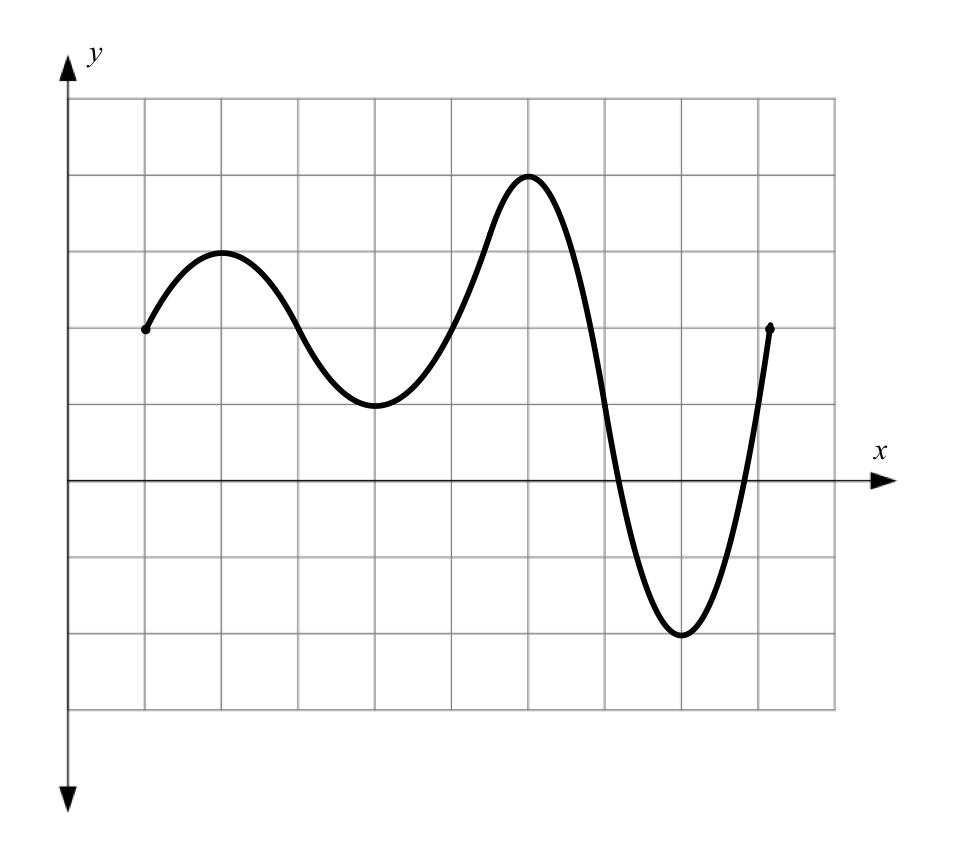
\includegraphics[width=2.5in]{Rolles1.png}
\end{figure}
\clearpage
\subsection*{Example 2} Verify that the function satisfies the three hypotheses of Rolle's Theoremon the given interval. Then find all the numbers $c$ that satisfy the conclusion of Rolle's Theorem.
\begin{enumerate}[label=(\alph*)]
    \item $f(x)=2x^2-4x+5$ on $[-1,3]$\vspace{5cm}
    \item $f(x)=x+x^{-1}$ on $[1/2,2]$\vspace{5cm}
\end{enumerate}
\subsection*{Example 3: Apply Rolle's Theorem}
\begin{enumerate}[label=(\alph*)]
    \item Prove that the equation $x^3+x-1=0$ has exactly one real root! \textit{Hint: First Use IVT}\vspace{4cm}
    \item Prove that the function $f(x)=x^3+e^x$ has exactly one real zero.
\end{enumerate}
\clearpage
\begin{tcolorbox}
\subsection*{Mean Value Theorem}
Let $f$ be a function such that
\begin{enumerate}
    \item $f$ is \underline{\hspace{3cm}} on the closed interval $[a,b]$,
    \item $f$ is \underline{\hspace{3cm}} on the open interval $(a,b)$
\end{enumerate}
then the conclusion is: there is a number $c$ in $(a,b)$ such that
\[
f'(c)=\frac{f(b)-f(a)}{b-a}\textrm{  this is equivalent to } f(b)-f(a)=f'(c)(b-a).
\]
\textit{In other words:} Given a continuous differentiable function on a closed interval, the secant line through the endpoints runs parallel to at least one tangent line at a point \underline{in} the interval.
\end{tcolorbox}
\begin{figure}[h!]
    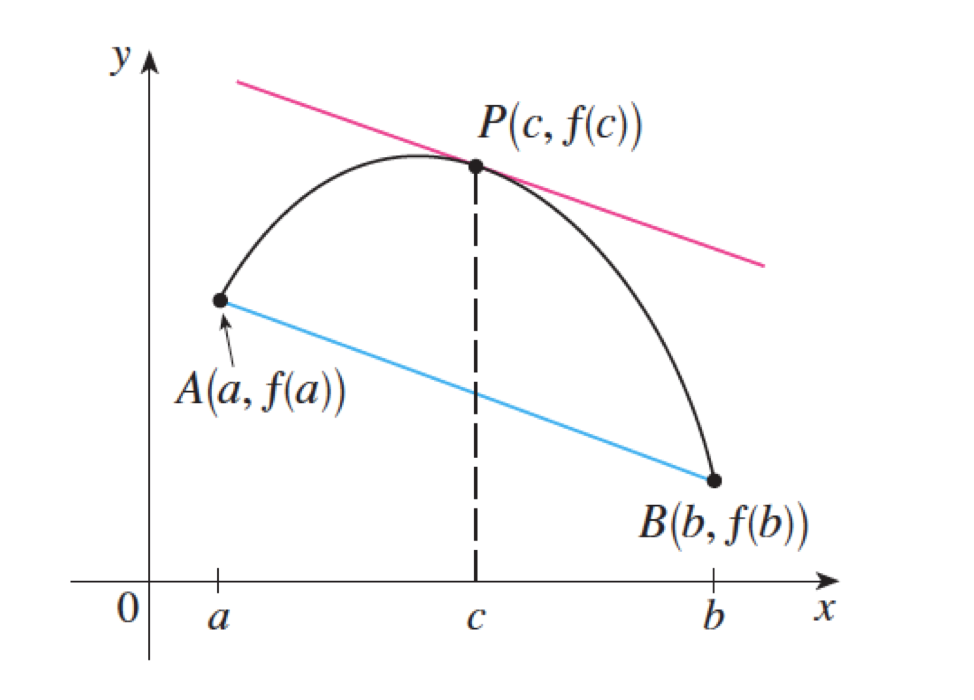
\includegraphics[width=3in]{MVT.png}
\end{figure}
\subsection*{Example 4} Verify that the function satisfies the hypotheses of the Mean Value Theorem on the given interval. Then find all numbers $c$ that satisfy the conclusion of the Mean Value Theorem.
\begin{enumerate}[label=(\alph*)]
    \item $
f(x)=\sqrt{x-1}\textrm{ on [1,5]}$\vspace{4cm}
\item $f(x)=\ln x\textrm{ on [1,e]}$
\end{enumerate}
\clearpage
\subsection*{Additional Examples}
\begin{enumerate}[label=(\alph*)]
    \item Consider $f(x)=x^3-x$ on $[0,2]$. Verify that $f$ satisfies the hypotheses of the Mean Value Theorem on the interval and find the values of $c$ that satisfy the conclusion.\vspace{4cm}
    \item Suppose $f$ is continous and differentiable and $f(0)=-3$, $f'(x)\leq 5$ for all $x$. How large can $f(2)$ be?\vspace{4cm}
    \item Does there exist a function $f$ such that $f(0)=-1$, $f(2)=4$, and $f'(x)\leq 2$ for all $x$?
\end{enumerate}
\end{document}